\documentclass[acmtog]{acmart}
\usepackage{listings}

\usepackage{makecell}
\usepackage{booktabs}
\usepackage{caption}
\usepackage{subcaption}
\usepackage{lmodern} 
\usepackage{amsmath} 
\usepackage{xcolor}  
\lstset{
	basicstyle=\ttfamily,
	columns=fullflexible,
	frame=single,
	breaklines=true,
}
\renewcommand\cellalign{tl}
\def\BibTeX{{\rm B\kern-.05em{\sc i\kern-.025em 
b}\kern-.08emT\kern-.1667em\lower.7ex\hbox{E}\kern-.125emX}}

\begin{document}

\title{Towards Detecting Stalkerware Through Network Traces}


\author{Audrey Randall}
\author{Hugh Feng}
\author{Yu-Wun Wang}
\affiliation{\institution{UCSD}}

\begin{abstract}
Intimate partner violence (IPV) is a pervasive problem that has been changed by 
the advent of the digital age. The ubiquity of smartphones has made it easy 
even for someone with no technical skills to perform surveillance of a device 
that they have access to. In the context of IPV, abusers often have access to 
the devices of their partners, and either know or can coerce the passwords to 
those devices. With such unrestricted access, an abundance of surveillance 
options exist, 
whether the goal is to track location, remotely block incoming calls or 
messages, record all communications, monitor browsing history, or lock a 
survivor out of their accounts. For some types of information, no extra 
software is required to gather it. For example, Facebook can reveal a user's 
location to their friends. Another example is Apple's backup service, which can 
make copies of text messages and call logs accessible to anyone with the iCloud 
credentials of the phone. Other types of control that might be attractive to an 
abuser, such as the ability to block incoming communication from certain 
people, require software to be installed on the target device. We refer to such 
software as ``stalkerware.'' Stalkerware is dissimilar to other forms of 
malware because of how easily the adversary can access the target device. 
Consequently, traditional assumptions about security do not apply to it, and 
traditional methods of studying it are ineffective. Antivirus, which can 
normally provide information about malware, is poor at detecting 
stalkerware.\cite{chatterjee_spyware_2018} Network Intrusion Detection Systems 
(IDSs) also have low detection rates. This lack of information results in many 
unanswered questions about the use of stalkerware in the context of IPV.

This work takes a step towards answering one of those questions: namely, 
\textit{how prevalent is stalkerware today?} We identify the traffic signatures 
of 24 stalkerware apps, with the goal of being able to identify it from a 
network operator's vantage point. We show that our signatures identify 
stalkerware with few false positives. Additionally, we present a simple method 
of generalizing the signatures we identify, and show that our generalized 
signatures also give few false positives. We also show that peculiarities of 
the stalkerware ecosystem may aid researchers in detecting it, and in 
generalizing specific network signatures to apps that have not been manually 
identified. The ethical and bureaucratic issues inherent in doing a large-scale 
measurement study on real traffic prevented us from using our signatures to 
estimate how much stalkerware exists in the wild. However, we present a plan 
for how we could move forward. 
\end{abstract}

\maketitle

\section{Introduction}
Intimate partner violence, or IPV, is a pervasive problem in the United States 
and elsewhere. One in four women and one in six men will be subject to some 
sort of intimate 
partner abuse during their lifetimes, where ``intimate partner abuse'' can 
include physical, emotional, or sexual abuse, as well as stalking or rape. In a 
world where technology now pervades every aspect of our lives, some 
aspects of IPV have changed too. Technology can now be abused in a variety of 
ways that harm survivors of IPV. Previous work \cite{ristenpart_ucsd_talk} has 
classified these into four categories of attacks: ownership-based, account or 
device compromise, harmful messages or posts, and exposure of private 
information. Ownership-based attacks are possible when the abuser owns the 
device used by the victim or the victim's children. They are then capable 
of installing software on it that can remotely destroy the device or prevent or 
monitor access and usage. Attacks based on account or device compromise are 
possible when the abuser does not own the device but nevertheless can guess 
passwords or compel the victim to reveal them, or has access to the unlocked 
device, or can remotely ``hack'' it using knowledge of security questions or 
passwords. Some examples of a ``harmful message'' attack include messaging the 
victim from a spoofed account, messaging the victim's family or friends, or 
impersonating the victim using their own accounts. Finally, attacks that expose 
private information can involve ``revenge pornography,'' revealing an HIV 
status, creating fake profiles offering sexual services, and blackmail. While 
some of these options (such as tracking a victim's location) are available to 
an abuser without installing any extra software on the phone, others are not. 
We refer to monitoring software that can record online activity, 
communications, and location, or remotely tamper with the device, as 
``stalkerware.''  

Stalkerware is not as widely studied as other types of malware, and much less 
information about it is available. There are a few key differences between it 
and other forms of malware. First, stalkerware is meant to be installed 
by someone with physical access to the target device, not remotely by 
exploiting vulnerabilities. In the 
context of intimate partner abuse, this presents an enormous 
threat, given how frequently the abuser has unfettered access to the target 
phone. Second, the 
threat model used by malware developers includes sophisticated antivirus and 
intrusion detection systems (IDSs). Both malware and stalkerware need to hide 
their presence on the target device, but malware is much more likely to 
attempt to obfuscate its network traffic to thwart these adversaries. 
Stalkerware does not: it does not 
need to. Most antivirus does not detect apps capable of monitoring a target as 
potentially dangerous \cite{chatterjee_spyware_2018}. This presents an 
opportunity to glean information about stalkerware that is not available in the 
study of other forms of malware. At the same time, it limits a researcher's 
ability to use information collected by antivirus as a source of information 
about stalkerware. Third, stalkerware falls 
for the most part into two categories: apps that are explicitly advertised for 
surveilling spouses and partners, and apps that have a different stated use but 
can be repurposed to stalk a target. These are usually marketed for theft 
prevention, finding lost devices, parental control of children, and employer 
control of employees. Previous literature refers to these as "dual-use" 
apps\cite{chatterjee_spyware_2018}. Some dual-use apps are ones that the 
victim wants to keep installed, such as 
``find my phone'' apps or social media apps that leak the user's location. The 
most troubling example of this is Facebook, which most victims want to keep 
so that they can contact their support network for help.  Determining if a 
particular dual-use app is being used for intimate partner surveillance (IPS) 
presents an enormous challenge. Given the wide spectrum of apps that can be 
used to facilitate IPS and the limited scope of this project, we chose to focus 
on more overt spyware.

Largely due to the differences between stalkerware and other malware, most 
available information on the \textit{pervasiveness} of stalkerware is anecdotal 
and piecemeal. Small-scale studies on how widespread spyware is do exist, but 
they have limitations. For example, in a survey of 72 
domestic violence shelters performed by NPR in 2014, 85\% said they worked with 
survivors whose abusers had tracked their location using their smartphone's 
GPS. 75\% said they have worked with clients who have had their conversations 
monitored by hidden stalkerware apps.\cite{shahani_smartphones_nodate} However, 
this study does not report how many individual clients experienced being 
digitally stalked. Additionally, it and similar work relies on 
reports from domestic violence shelters and health workers, which do not give 
a complete picture of the situation. Little to no data exist regarding spyware 
use on IPV victims who never visit a shelter. Traditionally, antivirus vendors 
collect metrics about 
malicious software, but antivirus often does not detect spyware 
\cite{chatterjee_spyware_2018}. Alarmingly, the stalkerware 
websites themselves claim to have hundreds of thousands of downloads per app, 
but these numbers are not likely to be trustworthy. The goal of this work is 
therefore to identify a means of identifying stalkerware in the wild so that it 
can be enumerated. We identified unique signatures in the traffic of 24 
stalkerware apps, by examining a traffic features such as domain names, HTTP 
header fields, protocol, and server name indicators (SNIs). For a complete 
list, see section \ref{network_signatures}. These signatures can be used by 
antivirus software and IDSs to determine how widespread stalkerware is. We show 
that these signatures are distinguishable from ordinary smartphone 
network traffic. We also propose a simple method of generalizing our signatures 
to spyware that we did not manually examine, and evaluate its robustness.


We began by identifying a set of apps that appear to be 
marketed primarily for IPS. We focused exclusively on Android apps, since our 
two test phones were both Androids. Apps that appear in Google searches for 
terms like 
"catch a cheating spouse," use vague language that appear to be marketed 
towards IPS, and label themselves as "spyware" became candidates that we 
considered. Overt spyware is not generally available from the app store - it 
must be downloaded from the manufacturer sites. It also costs much more than a 
typical app, with monthly 
subscriptions ranging from \$12 to \$70 per month. The exception is an app that 
we call SpyToMobile, which survives on the app store by frequently 
``reskinning'' itself (see section \ref{reskinning}).  
We selected several of overt apps to test. All of these apps brand themselves 
as spyware and advertise that their products are undetectable on the target 
phone, despite also having disclaimers in small text that their software should 
not be used for any illegal activity. Some use language that appears designed 
to appeal to abusers. For example, underneath one promotional 
video, the app TheOneSpy has the disclaimer: ``Note for this video: Don't 
confuse with the world `Loved Ones' as spouse or Girl friends! Word Loved ones 
has used for kids and teens.''\cite{noauthor_theonespy_2013} All of these apps 
advertise that once they are installed, they are in ``stealth mode'' and are 
completely undetectable. This is not entirely the case - they appear in the 
list of all applications, but take care to name themselves something innocuous 
such as ``Data Backup'' or ``System Service.'' None of the overt apps that we 
examined required rooting the phone. When installed, they ask for all the 
permissions they 
require, including device administrator privileges. They are then capable of 
blocking incoming calls, recording messages that have been deleted, recording 
the screen of the phone using accessibility features, monitoring apps such as 
Facebook, WhatsApp, Kik, and Viber, and more.

Other apps were explicitly intended as spyware, but nevertheless available from 
the Play Store. They fell into two categories: spyware that reskinned itself to 
appear to be many different apps, and apps designed for parents to keep track 
of children (or in one case, for adult children to track elderly parents.) For 
the most part, this latter category was offered by antivirus companies such as 
Avast and Norton. These apps offered 
multiple features, such as call screening, blocking Google search results, 
recording text messages and call logs, and ``panic buttons'' that would allow 
the surveilled phone to contact the surveillant and raise an alarm. They do not 
hide their app icons and generally make an effort to notify the user that the 
monitoring app is installed on their phone. The spyware that we found on the 
Google Play store that did \textit{not} notify users of its presence consisted 
of one app, which we call SpyToMobile after the title on its loading screen, 
that was provided on the Play Store under many different names (see section 
\ref{reskinning}). 

We also identified many apps that were designed to track location or text 
messages, but were less comprehensive than the overt spyware. They 
track one feature each instead of tracking location, communication, and 
browsing history all at once. For the most part, these apps were free and 
available on the Google Play Store. Most of them were designed to keep track 
of the locations of the users' friends. They tended to be ineffective - nearly 
all of the apps we found that did not work fell into this category. Most of 
these apps were unable or unwilling to hide their icons, and some provide an 
explicit notification that the app is in use, although this notification can be 
easily disabled in the Android notification settings. 

\section{Related Work}
Previous studies \cite{stories_from_survivors, burke_using_2011}, the media 
\cite{shahani_smartphones_nodate, chatterjee_spyware_2018}, and intimate 
partner violence (IPV) survivors \cite{ristenpart_ucsd_talk} have all reported 
that spyware is becoming an increasingly utilized means of performing
intimate partner surveillance (IPS). Tracking functions supported by spyware 
allow stalkers to monitor communications, track locations, and remotely 
activate cameras and microphones \cite{shahani_smartphones_nodate, 
chatterjee_spyware_2018}. Chatterjee et al. propose methods for searching for 
IPS-capable apps. By Google search query expansion and unsupervised 
classification, they collected 9,224 apps possibly related to IPS on Google 
play and the open Internet. They manually selected 70 apps for investigation. 
They observed the most fundamental functions of these apps are 
monitoring locations, communication logs and data, media contents, and phone 
usages. They also found that existing anti-spyware tools cannot effectively 
detect IPS-related apps \cite{chatterjee_spyware_2018}.
Mobile apps are often identified via the User-Agent string of the HTTP request, 
when one is available \cite{xu_identifying_2011}. With the increased use of 
HTTPS this may not always 
be the case, but we expect to find (based on conversations with authors of 
previous work) that security and best coding practices are not prioritized by 
stalkerware developers. Malware identification may be of use as well, 
since techniques are available to cluster malware that comes from the same 
source code into "families." \cite{hutchison_firma_2013}

\section{The Stalkerware Ecosystem}

We noted several interesting characteristics of the stalkerware ecosystem, some 
of which are beneficial to researchers attempting to identify stalkerware.

\subsection{The Practice of ``Reskinning''}
\label{reskinning}

\begin{figure*}
	\centering
	\begin{subfigure}{0.8\columnwidth}
		\centering
		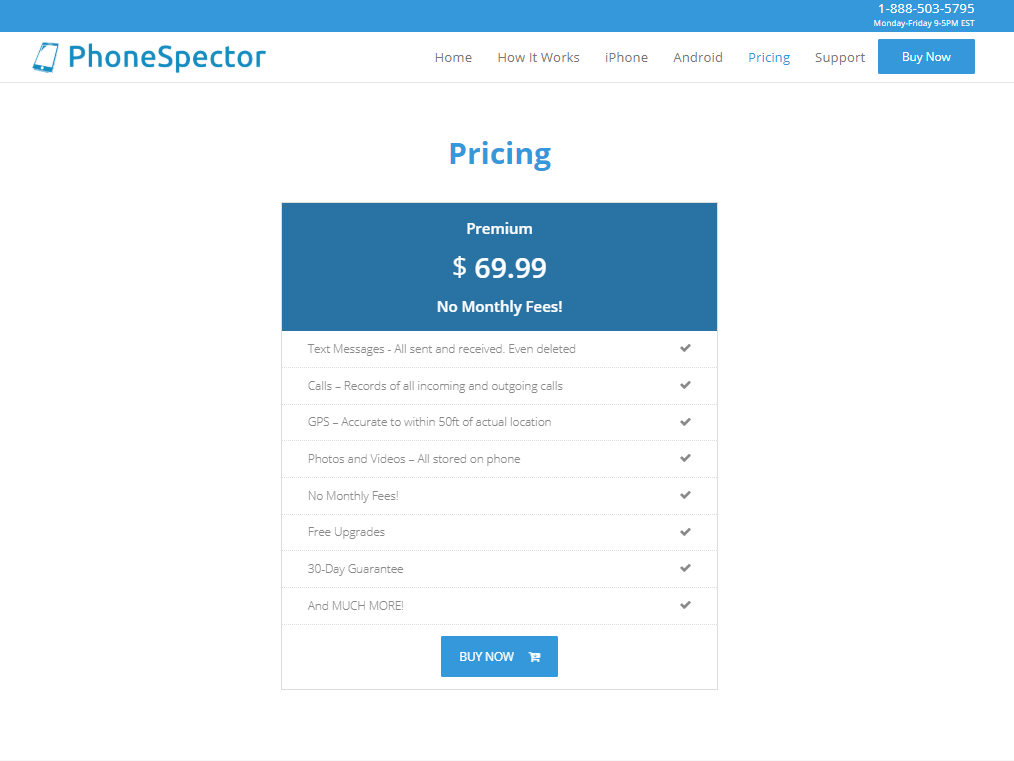
\includegraphics[width=0.9\linewidth]{../images/phonespector_small.png}
		\caption{PhoneSpector's pricing page }
		\label{fig:phonespector}
	\end{subfigure}%
	\begin{subfigure}{0.8\columnwidth}
		\centering
		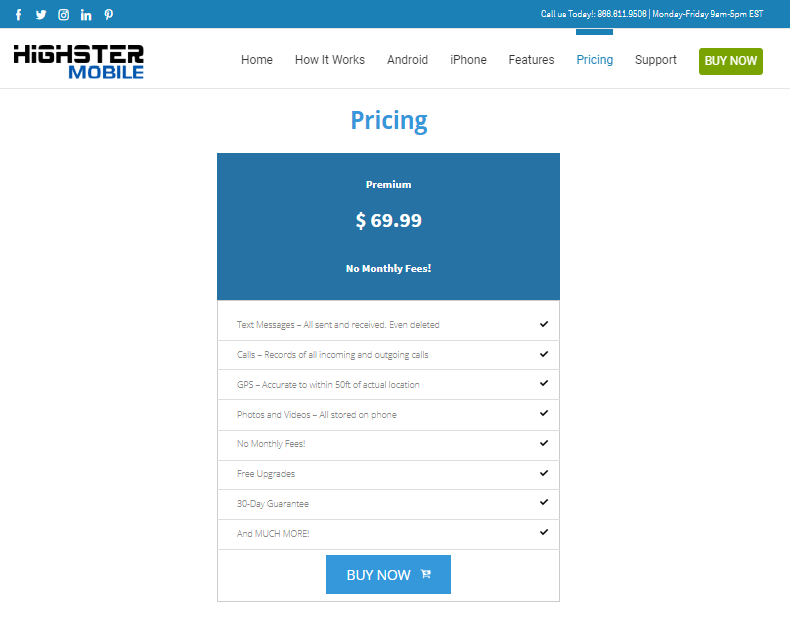
\includegraphics[width=0.9\linewidth]{../images/highstermobile_small.png}
		\caption{Highster Mobile's pricing page}
	\end{subfigure}
	\caption{PhoneSpector and Highster Mobile's payment pages. Although 
	PhoneSpector claims to be made by PhoneSpector LLC and HighsterMobile is 
	supposedly made by the Powerline Group, further investigation proved they 
	were the same company.}
	\label{fig:ilfmobiles}
\end{figure*}

\begin{figure*}
	\centering
	\begin{subfigure}{0.8\columnwidth}
		\centering
		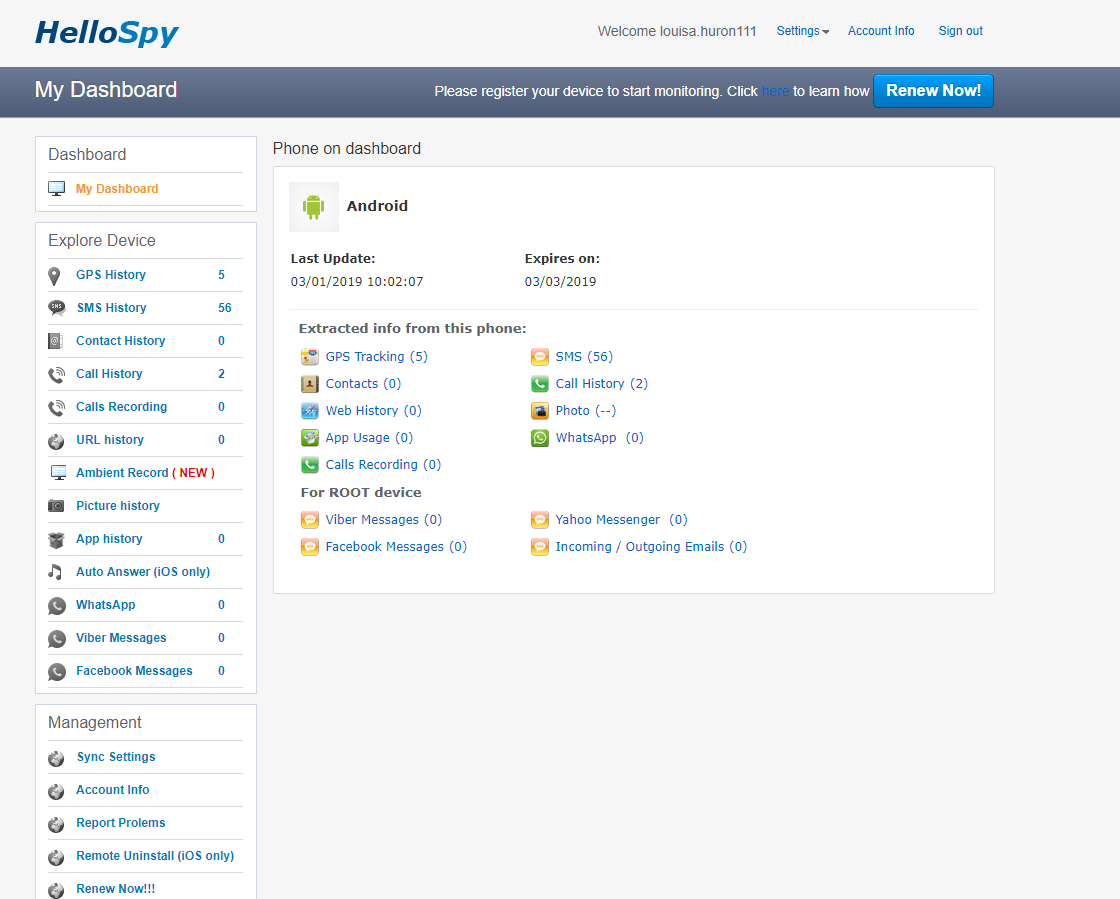
\includegraphics[width=0.9\linewidth]{../images/hellospy.png}
		\caption{HelloSpy's dashboard (cut off at bottom)}
		\label{fig:hellospy}
	\end{subfigure}%
	\begin{subfigure}{0.8\columnwidth}
		\centering
		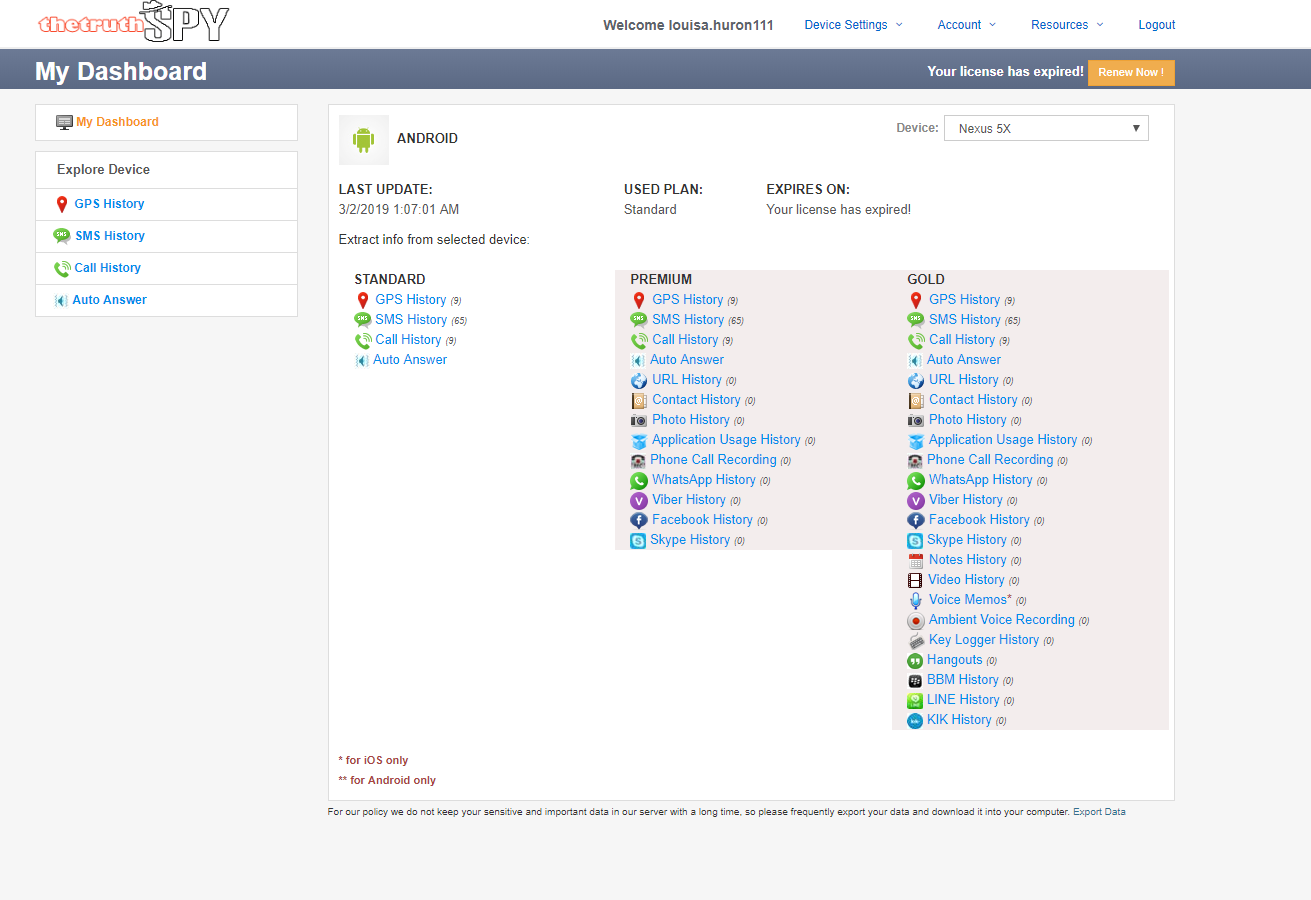
\includegraphics[width=0.9\linewidth]{../images/thetruthspy.png}
		\caption{TheTruthSpy's dashboard}
		\label{fig:truthspy}
	\end{subfigure}
	\caption{HelloSpy and TheTruthSpy have remarkably similar websites. Their 
	traffic signatures also turned out to be identical, leading us to believe 
	they are made by the same manufacturer.}
	\label{fig:hellospy_thetruthspy}
\end{figure*}

As previously mentioned, spyware has a high turnover rate on the Google Play 
store, which leads to a practice we refer to as "reskinning:" a single app will 
be posted under many names, icons, and manufacturer names. Presumably, 
manufacturers do this because spyware gets reported frequently and taken down - 
we have already seen one instance of a spyware app getting removed from the 
Play store while we were examining it. Overt stalkerware which is not available 
through Google Play has also turned out to use reskinning, for reasons we 
haven't yet discovered. Apps can frequently be identified as copies of each 
other by observing their dashboards (where users view the communications and 
locations of the target phones), download sites, and advertisements. Several 
groups of off-store apps have nearly identical websites, in terms of 
organization, color, fonts, placement of buttons, prices, and other factors. 
For example, the "ILFMobile group" consists of three different companies 
(ILFMobile, PowerLine Group, and PhoneSpector) that claim to make a total of 
four different apps. Their websites, however, were remarkably similar (Figure 
\ref{fig:ilfmobiles}). Further investigation showed that all three companies 
had the same physical address in addition to identical websites. Unfortunately, 
they also had identical bugs in their payment methods, so we were unable to 
purchase the apps and verify that their network traces were identical. Another 
example of stalkerware websites that appear to be strangely similar to each 
other in other ways is shown in Figure \ref{hellospy_thetruthspy}. This is 
admittedly somewhat circumstantial evidence - it is entirely possible 
that these manufacturers simply chose similar web templates, or copied each 
other's site in an attempt to undercut competition. We therefore confirmed our 
suspicions by checking if the traffic signatures were also similar, and found 
that they were. These reskinned programs are potentially a boon to 
our investigation as the identical network signatures make it more likely that 
one signature generalizes across multiple apps. We have identified the 
following groups of applications that appear to be reskinned versions of each 
other.
\begin{enumerate}
	\item \textbf{SpyToMobile group}: Employee Work Spy by Piter Cline, SMS 
	Tracker by TheHar, Mobile Tracking by Antwat, Cell Phone Tracker by Susdel, 
	and Texting, Chat, 
	Phone Spy by MaxLo. All of these apps download the same program, which is 
	called SpyToMobile. Any app from this group installed after the first 
	states ``SpyToMobile is already installed.''
	\item \textbf{ILFMobile group}: HighsterMobile, PhoneSpector, Auto Forward 
	Spy, Surepoint Spy, and EasySpy. We were unable to purchase these and 
	ensure that they have the same signatures due to a bug in their payment 
	system that prevented us from purchasing them.
	\item \textbf{Codero group}: HelloSpy and TheTruthSpy have identical 
	network signatures as well as nearly identical websites.
	\item \textbf{Spyzie group}: Spyzie and SpyMyFone also have identical network signatures 
	as well as similar websites.
	\item \textbf{CallSMSTracker group}: Call and Message Tracker by Remote 
	Karath and Cell Tracker by Trackme. These apps have identical dashboards 
	and contact the same domains.
\end{enumerate}
We cannot guarantee that we have identified all of the members of any 
particular group. If we have not, it will make other members easier to 
identify, since signatures we have already found will scale to identify more 
apps than we had time to download and manually examine.

\subsubsection{SpyToMobile}

\begin{figure}
	\centering
	\begin{subfigure}{0.5\columnwidth}
		\centering
		\includegraphics[width=0.9\linewidth]{../images/CellPhoneTracker.png}
		\caption{SpyToMobile's setup page }
		\label{fig:sub1}
	\end{subfigure}%
	\begin{subfigure}{0.5\columnwidth}
		\centering
		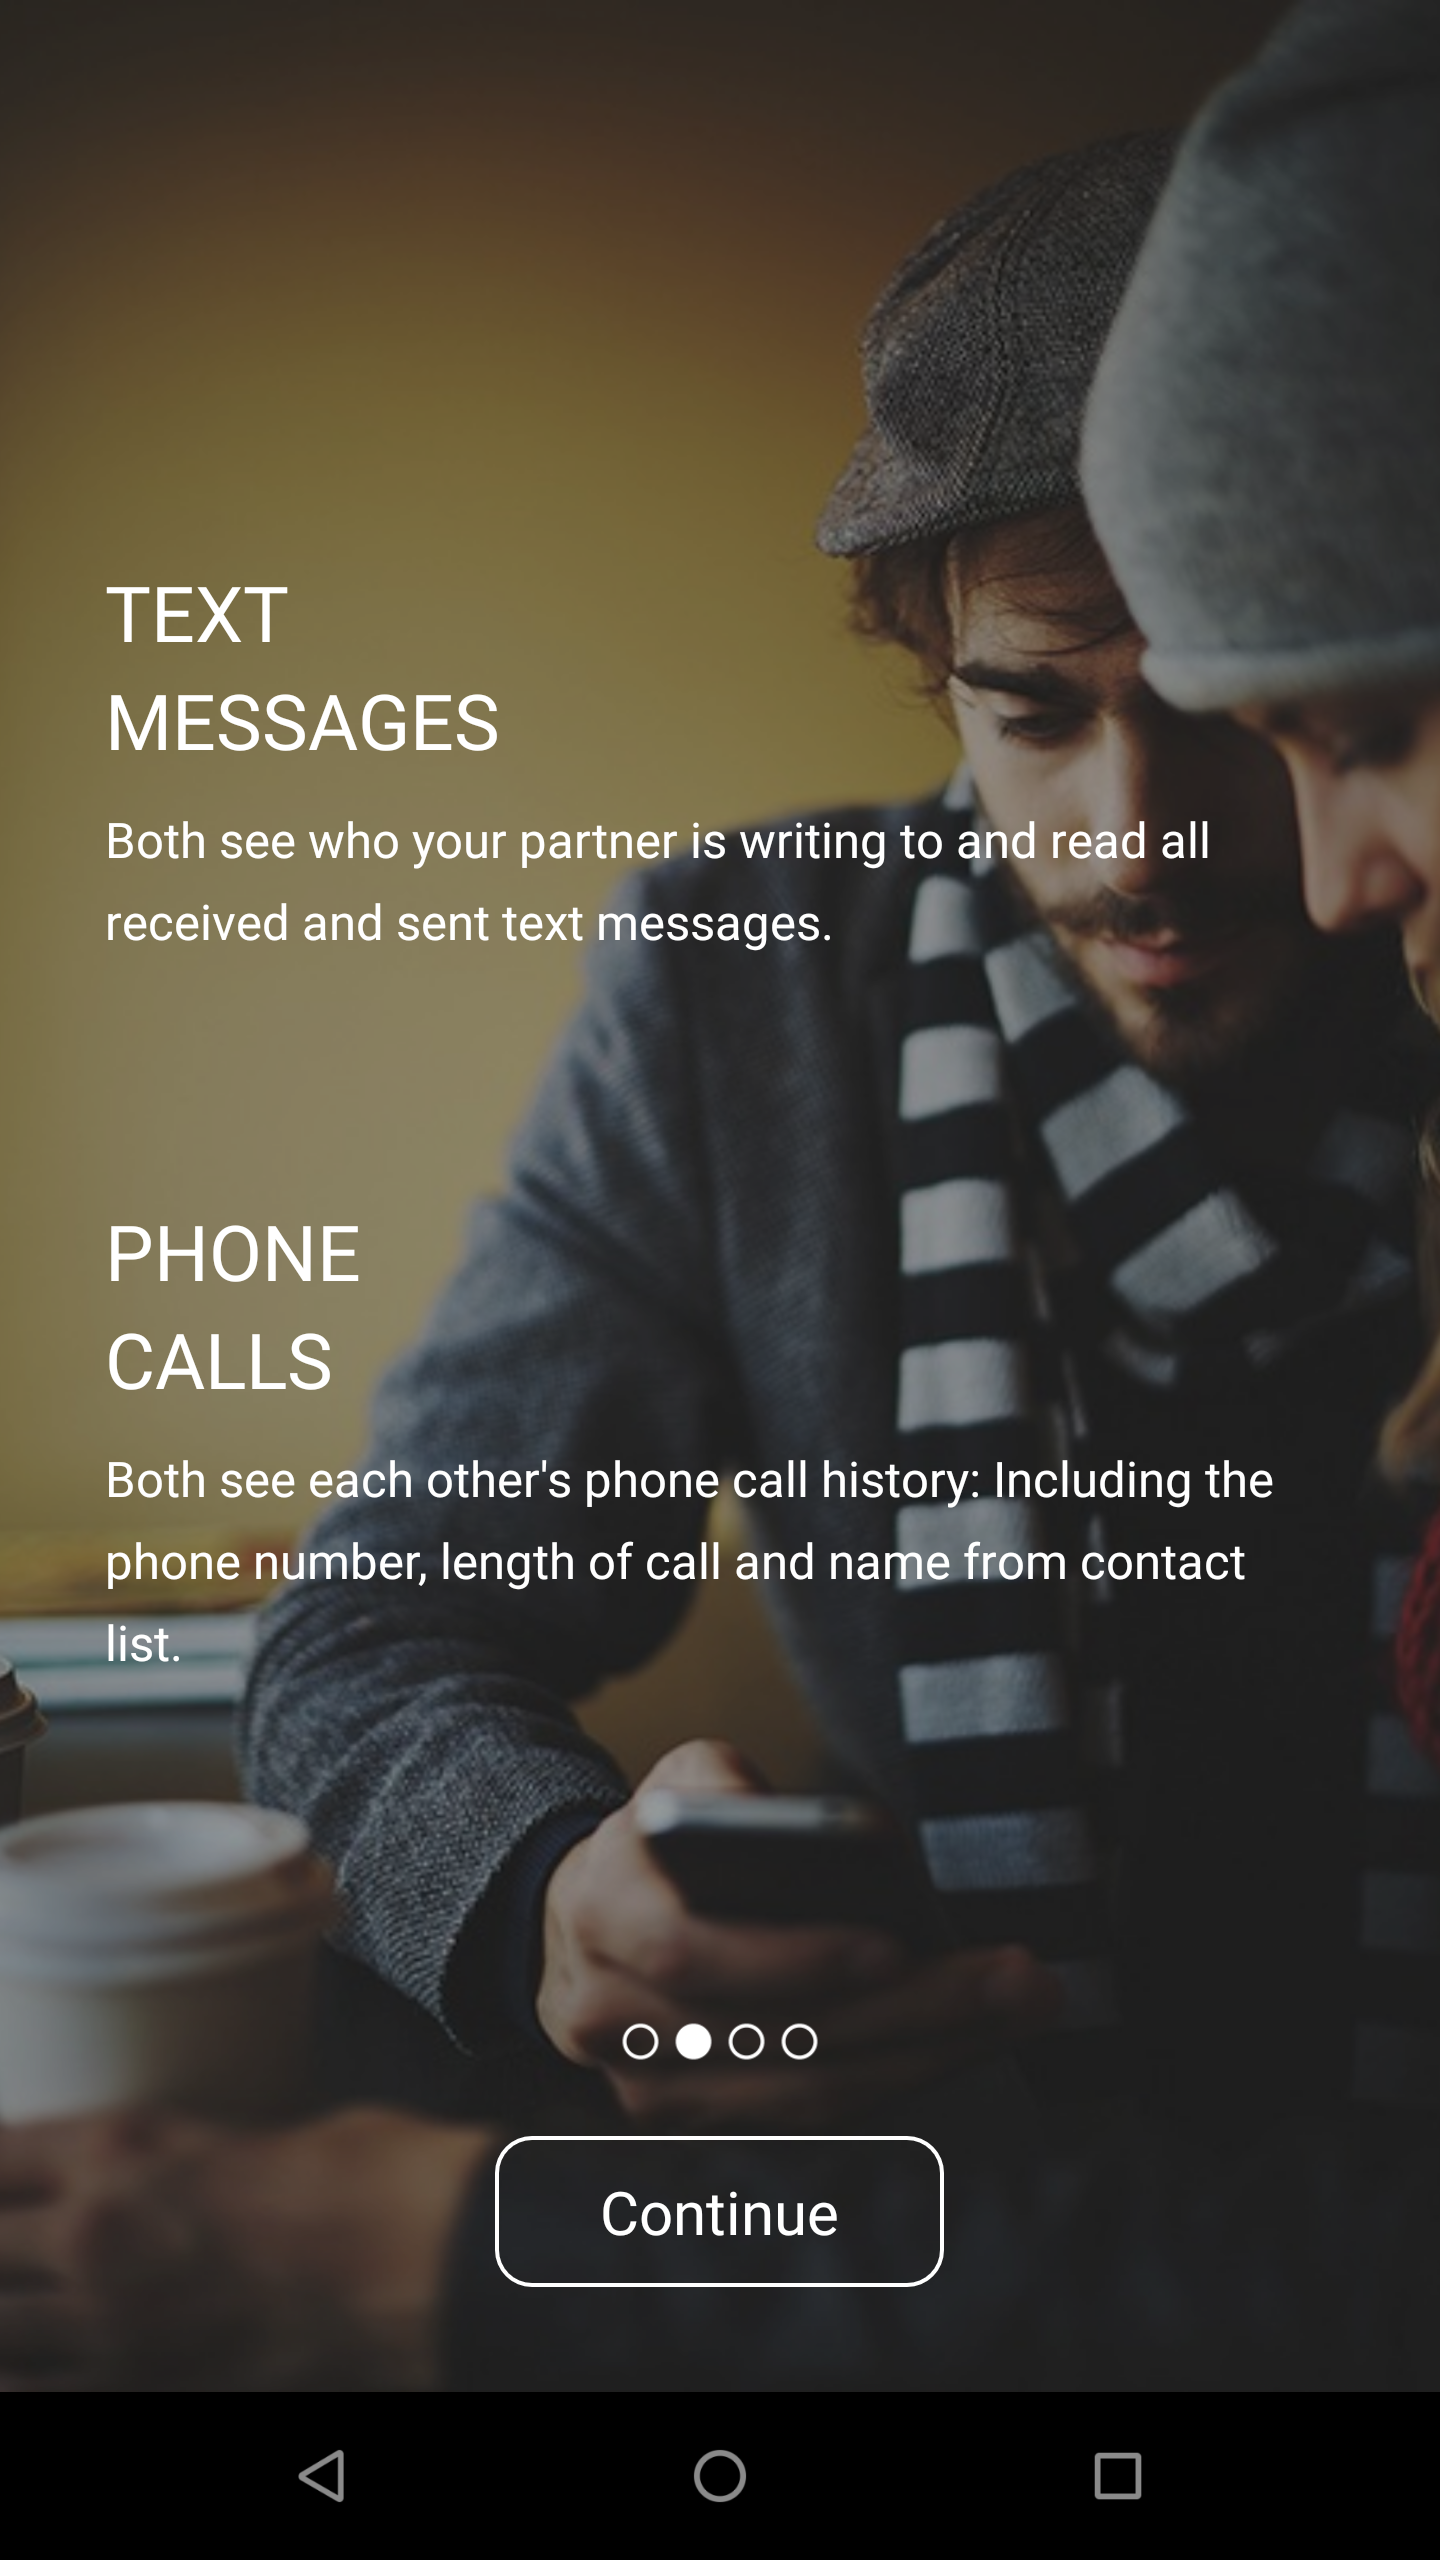
\includegraphics[width=0.9\linewidth]{../images/Couple_like_spy2mobile.png}
		\caption{A setup page for Couple}
		\label{fig:sub2}
	\end{subfigure}
	\caption{SpyToMobile and Couple's similarities. All SpyToMobile copies have 
	the same setup screen as \ref{fig:sub1} as well as identical signatures. 
	Couple did not share signatures with SpyToMobile.}
	\label{fig:spytomobile_couple}
\end{figure}


SpyToMobile is an interesting case 
because it fits the description of a generic stalkerware app so closely that it 
is the perfect example of spyware on the Play Store. Moreover, this single app 
has been repackaged multiple times. We have discovered that there have been at 
least six copies of the app on the Play store while our work has been ongoing, 
all with different developers and 
different names. We also found that the same image SpyToMobile uses in its 
"downloading" screen is used in another app, which had no similarities among 
its network signatures, called Couple. Figure \ref{fig:spytomobile_couple} 
shows the similarities.

\subsection{Competition Among Manufacturers}

App manufacturers appear to be well aware of their competition. When the term 
``hello spy'' is typed into Google Search, ads appear captioned ``Hellospy | 
See All Phone Data Remotely | mSpy.com'' and ``HelloSpy - Free Download | \#1 
Phone Tracker Software\&App | spymyfone.com.'' Clicking on these leads the user 
to the download pages for mSpy and SpyMyFone respectively, not the site for 
HelloSpy. Based on network traces and website appearances, we do not believe 
any of these three apps are made by the same manufacturer. Spyware groups also 
create "review" websites that review their own products, posing as third party 
spyware enthusiasts. At least one blog that is supposedly run by 
an independent party reviewed apps that coincidentally were all made by the 
ILFMobile group\cite{noauthor_best_nodate}. This blog reviews the 
"top 5 cell phone spy apps," all of which are ILFMobile's own apps, on a 
website called "bestcellphonespyapps.com." We haven't determined what advantage 
spyware manufacturers derive from appearing to make more apps and competing 
with themselves.

\subsection{Does Stalkerware Download Other Malware?}

Most free stalkerware appears to exist to serve advertisements. We only saw one 
instance of an app that came packaged with other malware, which in this case 
was a cryptominer for a cryptocurrency called Kin Coin.

We also observe a strange phenomenon among at least two of the paid, overt 
spyware apps. Both claimed that they had stopped working after two or three 
days even though they still appeared to be updating, and asked the user to 
click on a link to check if the app was still active. In one case, the URL of 
this link appeared to indicate that it would always claim the app had stopped 
working. The site would then request that the user re-download the app. We were 
confused as to why these apps would do this. 
The version of the app that was downloaded the second time appeared to be the 
same as the version downloaded first, and if the manufacturer wanted to 
download malware onto the phone, they could just do so with the first 
download. Nevertheless, our strongest explanation for this behavior is still 
that the false warnings were intended to convince users to download malware. We 
leave the task of determining if this was truly the case to future work.


\subsection{App Quality}

Free stalkerware apps vary widely in quality. Many simply don't work, or claim 
for some reason that they will only begin to work when the SIM card of the 
phone is replaced. Multiple apps that claim to track location instead just 
return the location associated with the phone's area code. A pair of others 
appeared to guess randomly - one reported that a device in San Diego was in 
Fawn Creek, Kansas, and another reported the same device was in Detroit, 
Michegan. Another common glitch was for spyware that records texts to only 
record one participant's side of the conversation. Their main purpose seems to 
be to serve advertisements - we did not 
catch any of the non-functional apps contacting domains associated with malware 
(except when the app itself was marked as malware). 

\section{Methodology}

\subsection{Finding Apps}
We selected thirty apps from a list provided by the team of Cornell researchers 
who performed the original large scale study of 
stalkerware\cite{chatterjee_spyware_2018}. An 
additional fifteen apps were included because they were recently added to the 
Google Play store, or to replace apps that were found not to function. We found 
these apps simply by searching for them using keywords such as "spy" or 
"track." Encouragingly, specifically IPV-related search terms 
such as "track girlfriend" return no results on the Play store. On the other 
hand, that did not mean stalking apps were not available on the play store, it 
just meant that different search terms had to be used to find them. We selected 
a diverse set of purposes, from explicit spyware to innocuous dual-use apps. We 
predict that the apps we chose are likely to be 
downloaded when an abuser without deep technical knowledge tries to install 
stalkerware, since they are either among the first results upon searching for 
stalkerware, or are well advertised as spyware.

We recognize that there are possibly hundreds of apps on the market that can be 
repurposed as stalkerware. Therefore, any useful process for identifying 
network signatures will eventually have to cover far more apps than we are 
starting out with. Our mere forty-five apps barely scratch the surface of the 
ecosystem, so they may not provide a representative sample. Therefore, 
we did not employ any vigorous app selection methods, since we know this is 
just a starting point. Our hope is to eventually find a way to partially 
automate the signature identification process.

\subsection{Experimental Setup}
Out of the 45 apps we searched for for, 36 still existed on the app store. We 
installed these one at a 
time on one or both of two test phones, a Nexus 5X and a Nexus 6P. These phones 
were chosen simply because they were readily available. Stalkerware user 
models  fall into two types: either 
a login to a web portal is provided for the attacker to view the data, or 
the app comes with an ``attacker'' app and a ``target'' app, and the attacker 
app must be installed on another phone.

After installing an app, we first confirmed that it was functional and capable 
of acting like stalkerware. 
We then began tracking the phone's network traffic using Wireshark. For the 
majority of the apps, a network trace 
of five to ten minutes is enough to detect traffic going to and from the 
stalkerware app as long as the functions the app tracks like text or GPS are 
in use or the tracker app has manual update capabilities. We then manually 
examined the traffic, isolated that which belonged to the app, and determined 
the signature.

\subsection{Ethical Considerations}

We created two aliases in order to avoid exposing any personal information to 
an ecosystem that is notorious for mishandling it\cite{ristenpart_ucsd_talk}. 
It is likely that the privacy of victims is 
not a high priority for anyone prepared to monetize abusive relationships, and 
stalkerware manufacturers have leaked victims' information in the past 
\cite{koebler_stalkerware_2018, franceschi-bicchierai_this_2019}. We took 
precautions by deleting all personal 
data that had been on the phones at the start of the project. However, we were 
not quite cautious enough - the app SpyMyFone managed to scrape a list of 
deleted contacts off of the Nexus 5X. As of this moment, we do not know how. We 
have deleted the account and requested that SpyMyFone delete all information 
associated with it from their records, but we have no evidence that they have 
complied. This served as a valuable and sobering lesson for the future.

The original goal of this project was to identify traffic signatures so that 
they could be detected by an IDS (Intrusion Detection System) or a network 
tap in an anonymized fashion. We hoped to use differential privacy techniques 
such as Google's RAPPOR algorithm \cite{erlingsson_rappor:_2014} to collect 
aggregated statistics about stalkerware use, while denying ourselves the 
ability to identify any particular device that had stalkerware installed. Upon 
further investigation before we began the project, this turned out to be 
insufficient protection. We do not have the expertise required to assist 
victims of abusive 
relationships or domestic violence. If we were to uncover evidence of 
stalkerware, it is unclear what we should or could do with that information. We 
chose not to take our research in this 
direction to avoid causing any unintended harm. We limit ourselves to 
identifying traffic signatures on apps that we installed on personal phones. We 
leave the question of deploying our signatures to later work, once we have 
developed partnerships with experts who can advise us.

Wiretapping the phones was accomplished by setting up our personal computers as 
WiFi hotspots. Since we controlled the passwords required to connect to our 
networks, and Windows alerts the user when a device connects to its mobile 
hotspot, we were able to ensure that we did not tap any traffic other than that 
of the test phones. 
\section{Results}

\subsection{Network Signatures}
\label{network_signatures}

We identified the following traffic features as candidates for network 
signatures.
\begin{itemize}
	\item Application Layer
	\begin{itemize}
		\item HTTP
		\begin{itemize}
			\item Packet content
			\item User-Agent
			\item Presence of unique header fields 
			\item Packet length
			\item URI
			\item Host Name
		\end{itemize}
		\item Presence of excessive number of location requests
	\end{itemize}
	\item Transport Layer
	\begin{itemize}
		\item TLS 1.2
		\begin{itemize}
			\item Server Name Indicator
		\end{itemize}
		\item TCP
		\begin{itemize}
			\item Ports
		\end{itemize}
	\end{itemize}
	\item Internet Layer
	\begin{itemize}
		\item IP address
		\item Reverse-DNS-lookup domain name
	\end{itemize}
	\item Other
	\begin{itemize}
		\item Packet frequency
	\end{itemize}
\end{itemize} 

Some of these features did not prove to be easy to use as signatures.
For example, different types of stalkerware exhibit wide variance in how often 
they send updates back to their servers. Some apps advertise 
``real time'' tracking, where new texts are uploaded to the service as soon as 
they are sent by or arrive at the phone, and location is updated as soon as the 
phone moves. In our experiments, very few of the apps who claimed this ability 
actually delivered on their promise. Texts were uploaded anywhere between ten 
minutes to a day after they were sent. Some of the stalkerware dashboards 
included a button that would update or refresh the data, but this usually did 
not trigger traffic to be sent from the phone.

Another feature we failed to identify was the presence of unusually high 
numbers of location requests. Since phones can (if GPS is not available) get 
information about their location by seeing which WiFi AP they are connected to, 
we attempted to identify packets that were requesting location from the AP, but 
were unsuccessful.

All of the other features proved to be useful in identifying some subset of the 
apps we examined. 

\subsection{Traffic Results}

The majority of stalkerware apps communicate though HTTP or HTTPS. A minority 
use less common protocols, such as the app that could turn a phone into a live 
video camera remotely, which used STUN. We examined the features listed above 
for each app and tried to isolate some subset of them that we believed would be 
unique enough to identify that traffic. For the majority of the apps, the 
domain provided by a reverse DNS lookup was sufficient. This supported our 
assumption that most stalkerware does not attempt to obfuscate its traffic. 
Even servers hosted on Amazon's AWS had unique domain names, which usually 
consisted of some string identifying the app prepended to a string identifying 
which AWS datacenter the app is hosted by. We found signatures for 24 out of 
the 45 apps we examined. Of the remainder, nine were removed from the Google 
Play store before we began the project, and twelve either didn't work as 
stalkerware or didn't work at all.

\subsection{Generalizing Signatures}
\begin{table*}
	\begin{tabular}{p{6cm}p{4cm}p{4cm}}
		\toprule
		Generalized Signature & Unique Apps & Total Apps \\
		\hline
		Domain contains "spy," "track," "find" & 6 & 12 \\
		SNI contains "spy," "track," "find" & 6 & 6 \\
		User-Agent contains "spy," "track," "find" & 1 & 3 \\
		User-Agent contains known app name & 1 & 1 \\
		Domain contains known app name & 3 & 4 \\
		SNI contains known app name & 1 & 1 \\
		SNI contains known app manufacturer & 3 & 3 \\
		Domain contains known app manufacturer & 3 & 3 \\
		\midrule
	\end{tabular}
	\caption{Generalized signatures, created by identifying the similarities 
		between specific signatures}
	\label{tab:gen}
\end{table*}
Since the 24 apps that we manually identified signatures for undoubtedly 
represent a small proportion of all of the stalkerware available, we next 
attempted to look for patterns our signatures had in common that would allow us 
to generalize them. To our surprise, this was relatively straightforward.  
For example, the words "spy," "find," and "track" appeared frequently in 
various fields of the traffic. The most common place to find them was in the 
destination domain, which we found using Wireshark's reverse DNS lookup tool. 
12 of the 24 apps that we eventually found signatures for contained these 
spyware keywords in their domains. We therefore labeled this signature the 
``keyword method.''

For the apps whose traffic do not contain "spy," "find," or "track," we 
next check for the app name, the manufacturer name, or substrings of either. 
Using these indicators has a significant disadvantage - we must be certain that 
the app is stalkerware and that the manufacturer doesn't make anything except 
stalkerware. In the case of smaller apps and reskinned apps, this may actually 
be a reasonable assumption. Manufacturer names are generated to fool the 
Google Play store into thinking the app is new, not to identify a real company, 
and are therefore unique by necessity. We note that the two apps we can only 
identify by manufacturer are made by GPSWOX and GeoZilla. GPSWOX makes 
location-tracking apps of all kinds, some of which may be difficult to use as 
stalkerware, but GeoZilla's only apps are all designed to track a phone. Since 
only two apps were identified this way, the false positive rate should be 
investigated further. 

The generalized signatures shown in Table \ref{tab:gen} can be used to identify 
all but three (12.5\%) of our apps given nothing but information available on 
the Google Play store. This means that if we were able to reliably identify 
apps on the 
Play Store than can be used as stalkerware, it would be possible to identify 
the traffic of a large fraction of them without having to manually find their 
signatures.


\section{Evaluation}

We evaluated both specific and general signatures by taking twenty-four hours 
of network traffic captures on our own personal phones. Our goal was to 
determine a lower bound for our false positive rates. These 
captures also included periods of time that were deemed high risk for false 
positives as they emulated behavior that is most likely to be caught by our 
signatures. Given the relatively small amount of data we have to work with, our 
results should be considered extremely conservative lower bounds on the true 
false positive rates of our signatures. TODO: explain how we got false pos rate

Using the specific signatures, our false positive rate was zero. This is to be 
expected as we are very sure that there 
are no stalkerware apps installed on our personal phones and the filters used 
are quite specific to the apps that we looked at. 

Using the generic filters, we identified two TCP streams and 3 domains out of 
our total of 2869 streams and 1756 domains in our self network capture. In 
addition, these filters will only catch 21 out of the 24 apps that comprise the 
specific filter. This is an issue as it does infer that our generic filters are 
too generic. Upon looking at the specified domains, we see that these are most 
likely adware services that track user browsing data. Although there is a 
possibility that these can be considered malicious enough to add to our 
results, these are not stalkerware and as such count towards our false positive 
rate. Also while the percent of false positives is quite low, if we were to 
deploy this filter in an actual router, it would undoubtedly collect far more 
domains than we should be catching.

While looking at domains and TCP streams gets a good sense of how our filters work in a router, ideally we would also want to see how many apps we misclassify using our generic method. This is because our study is based on stalkerware in phones, and we make no assumption that stalkerware is only on cellular devices. Since we currently cannot connect each domain or TCP stream with a single app without identifying and tracking the traffic for all of our own apps, we make the assumption that each app will connect to only one domain, with the exception of the web browser. Using this assumption, we see that none of the apps on our phones are caught by our filter. Moreover, even apps meant for tracking buses do not get caught by the filter, despite the obvious connection that one could make. 





\section{Future Work}

In the future, we would like to automate our process. Ideally we would like to use machine learning to produce signatures for apps we have deemed stalkerware and any of it's copies. Moreover, when we have enough signatures to comprise a training and validation set, we can apply machine learning to fuse these signatures into a compact filter. This would likely be a good amount of work, but if it could be created it would make most stalkerware not in our dataset easily detectable.

Previously, we had expressed an interest in seeing if the signatures we found 
by hand could identify more apps without manual inspection. There are (as far 
as we can see) two possible methods of doing this. The first is to 
auto-generate signatures based on a list of keywords that commonly appear in 
domains, SNIs, User-Agents, and HTTP host names for stalkerware traffic. These 
keywords might include the names of the apps, substrings that appear in the app 
names, and words that seem relevant to tracking apps. A more complicated method 
would be to set up bots that can download potential spyware by searching 
various terms on the app store like "tracker app." The bots would have to run 
the apps and monitor their traffic, identifying app traffic by eliminating 
traffic from other sources. The remaining traffic would belong to the app, and 
the domains, SNIs, user-agents, and any other available identifying features 
could be recorded. However, the most difficult problem in this case becomes 
determining which apps are actually stalkerware on the app store, which is 
beyond the scope of this project. 

Additionally, we would like to actually test our signature on real word traffic. We are unable to do so currently since our method currently requires a network capture, and we do not have nor are able to get consent from everyone who uses a given network router. Hopefully we would be able to clear away these considerations in order to find the actual false positive rate of our packet filters.

\section{Conclusion}

Stalkerware is a problem, in the context of both society and security. As a tool for partner abuse, its use needs to be prevented before it can cause physical or mental harm, otherwise people cannot trust cell phones for their safety. As a software, current methods are unable to detect stalkerware on any given phone, the method of installation also exposes a security vulnerability that can be exploited for other purposes. In this paper, we have created a method that uses the intrinsic requirement of stalkerware, network communication, to detect it's presence on any device we can link to an IP address. This novel method is able to distinguish stalkerware traffic despite its relative simplicity.

Overall, we find that our method provides a much higher chance of detection than current antivirus software or IDS. We believe that this method can be expanded upon to be either more accurate or more inclusive. This method does have issues that prevent it from actual deployment, however it provides a good step forward in detecting stalkerware.

\bibliographystyle{ACM-Reference-Format}
\bibliography{IPS_Measurement}

\appendix
\clearpage
\begin{table*}
\section{Apps and Signatures}
\begin{tabular}{p{5cm}p{5cm}p{5cm}}
	\toprule
	App & Signature & Relevant Info \\
	\midrule
	HelloSpy & \makecell{HTTP Post to\\ <numbers>.dedicated.codero.net} & Same as TheTruthSpy HTTP \\
	
	TheTruthSpy & \makecell{HTTP Post to\\ <numbers>.dedicated.codero.net\\ User agent has hellospy in it} & Same as HelloSpy HTTP \\
	
	SpyMyFone & \makecell{HTTP 101 Switching Protocols\\ response\\
	Domain: data-api.spymyfone.com\\SNI my.spymyfone.com.\\
	Domain: ws.spyzie.com\\SNI ws.spyzie.com\\
	Domains: app-api.phonedata.me\\ws.phonedata.me\\
	SNI with unknown domain:\\ app-api.phonedata.me} & Uses WebSocket protocol and HTTP with User agent=aliyun-sdk-android/2.3.0/Dalvik/2.1.0 (Linux; U; Android 7.1.2; Nexus 5X Build/NJH47B \\

	Spyzie & \makecell{The same as SpyMyFone.\\ We are sure that SpyMyPhone\\ talks to spyzie.com} & Same as SpyMyFone \\
	
	iSpyoo & probably same signatures as HelloSpy and TheTruthSpy given identical websites, but apk is broken & Nonfunctional \\
	
	mSpy & \makecell{POST to pipe.thd.cc\\
	PUT to a18.dav.mspyonline.com\\
	Domain: apiv4.alter757.info} & HTTPS \\
	
	SMS Tracker (TheHar) & \makecell{Domain:uploads.spy2mobile.com\\ Domain contains sap4mobile} & spytomobile group (does NOT use HTTPS) \\
	
	SMS Tracker TM & \makecell{Domain:cust-198-154-111-218.\\corexchange.com \\ SNI:messages02.smstracker.com} & Only tracks text. HTTPS \\
	
	Find My Friends & Domain:production-finderapps-lb-1188906093.us-east-1.elb.amazonaws.com & HTTPS\\
	
	Avast Anti-Theft & domain:Antitheft.ns1.ff.avast.com& HTTPS. High packet counts\\
	
	Family Locator by ZoeMob & SNIs: celulocen.zendesk.com, api.familysafetyproduction.com
	Domains: proxy.vip.pod5.iad1.zdsys.com, www.zoemob.com & same as Life360
	HTTPS \\
	
	Couple Tracker -Mobile monitor & 162-144-96-67.unifiedlayer.com & HTTPS \\
	
	Call and Message Tracker -Remote karanth & \makecell{SNI=www.callsmstracker.com
	\\Domain contains onlinehome-server} & Similar to Cell Tracker, but uses HTTPS instead of HTTP \\
	

	
\end{tabular}
\end{table*}

\begin{table*}
	\begin{tabular}{p{5cm}p{5cm}p{5cm}}
		\toprule
		App & Signature & Relevant Info \\
		\midrule
		Mobile Surveillance and Security
		by Trackview & \makecell{HTTP req:\\ "GET /create\_session HTTP/1.1"\\ 
		User agent:test \\Host:relay.google.com\\
			Domains: relay.l.google.com,\\ stun.l.google.com} & Uses STUN 
			protocol \\
		
		Norton Family parental control & \makecell{domain: 
		spoc-muw1.norton.com,\\spoc-mue1.norton.com\\
			User-Agent: NOF/4.9.2.12/Android/8.1.0\\
			SNI: family.norton.com} & HTTP POST with protobufs, or TLS. \\
		
		Senior Safety App & \makecell{POST to 
		\\97.logger.mobi/signalr\_v1/<stuff>\\
			97.logger.mobi/auth/token} & requires payment\\
		
		Invisible Mobile GPS Tracker by
		GPSWOX.COM & \makecell{SNI:dn.gpswox.com\\ 
		Domain:gpswox.\\llcspnavigatio.netdna-cdn.com} & HTTPS \\
		
		Family GPS Locator by GeoZilla & 
		\makecell{Domain=static.<some-ip>.\\clients.your-server.de\\
			SNI contains geozilla w/ aws domains} & NOT HTTPS (wrong ports), 
			but TLS \\
		
		Phone Tracker By Number/Phone Tracker Family Locator & 
		http://66.147.232.135:8080/signalr & HTTP \\
		
		Automatic Call Recorder & \makecell{Domain: 
		http://winner-lb2-\\f918b4c7bf5ab40c.\\elb.us-east-1.amazonaws.com/ }& 
		HTTPS \\
		
		Find my Kids: Child GPS-watch and phone tracker & server name 
		api.findmykids.org & Talks to yandex.net? Russian something. 
		HTTPS \\
		
		Live Mobile Number Tracker & \makecell{GET with host=clk.trkmobi.net\\
			SNI track.56txs4.com, no domain\\
			Domain cs156.adn.rhocdn.net\\ with SNI req..startappservice.com,\\
			domain cs1112.wpc.rhocdn.net\\ with SNI info.startappservice.com} & 
			No actual tracking functions. Sets your location to Fawn creek, KS 
			\\
		
		track my phone pro & Domain:trackmyphones.com & HTTPS from the website, 
		HTTP over TLS from the app \\
		
		Cell Phone Tracker & Domain:spy2mobile.com & SpyToMobile lookalike \\
		
		Cell Tracker - Trackme & Domain:Onlinehome-server.com
		SNI:www.callsmstracker.com & Similar to Call and Message tracker. Sends 
		a post to a separate service. \\
		
		Texting, Chat, Phone Spy by Maxlo & Domain:spy2mobile.com & SpyToMobile 
		lookalike \\
	\end{tabular}
	
\end{table*}
\clearpage

\section{Wireshark Display Filters for Specific Signatures}
\begin{lstlisting}
ip.host contains dedicated.codero.net 
|| http.host contains hellospy
|| (ip.host contains data-api.spymyfone.com && ssl.handshake.extension.data 
contains "my.spymyfone.com") 
|| (ip.host contains ws.spyzie.com && ssl.handshake.extension.data contains 
"ws.spyzie.com") 
|| ip.host contains data-api.spymyfone.com 
|| ip.host contains ws.spyzie.com 
|| ip.host contains phonedata.me 
|| ssl.handshake.extension.data contains "phonedata.me" 
|| ip.host contains apiv4.alter757.info 
|| ssl.handshake.extension.data contains "thd.cc" 
|| ip.host contains thd.cc 
|| ip.host contains mspyonline.com 
|| ip.host contains corexchange.com && ssl.handshake.extensions_server_name 
contains messages02.smstracker.com 
|| ip.host contains life360.helpshift.com 
|| ip.host contains antitheft.ns1.ff.avast.com 
|| (ip.host contains production-finderapps && 
ssl.handshake.extensions_server_name contains "api.familysafetyproduction.com") 
|| ip.host contains production-finderapps 
|| ssl.handshake.extensions_server_name contains "celulocen.zendesk.com" 
|| ip.host contains www.zoemob.com 
|| ip.host contains unifiedlayer.com 
|| http.host matches "callsmstracker" 
|| ip.dst_host matches "onlinehome-server" 
|| (ip.dst_host matches "spoc-mu(|w|e)1.norton" && http.user_agent matches 
"(android|ios)")
|| ssl.handshake.extensions_server_name matches "family.norton" 
|| (udp && ip.host contains stun.l.google.com) 
|| http.host == relay.google.com && http.user_agent matches test 
|| http.host matches "97.logger.mobi" 
|| ssl.handshake.extensions_server_name matches "gpswox" 
|| ip.dst_host matches "gpswox" 
|| ssl.handshake.extensions_server_name matches "geozilla" 
|| ip.dst_host matches "clients.your-server.de" 
|| (ip.addr == 66.147.232.135 && tcp.port == 8080 && http.request.uri contains 
"signalr") 
|| ip.addr == 66.147.232.135 && tcp.port == 8080 
|| ssl.handshake.extensions_server_name matches "findmykids" 
|| ssl.handshake.extension.data contains "findmykids"  
||  ip.dst_host matches "(trackmyphones.com)" 
|| http.host matches "callsmstracker" 
|| ip.dst_host matches "onlinehome-server" 
\end{lstlisting}

\section{General Signature Wireshark Display Filters}

\begin{lstlisting}
http.host matches 
"(spy|track|find|antitheft.ns1.ff.avast|zoemob|life360|family.norton|gpswox|geozilla)"

|| ssl.handshake.extensions_server_name matches 
"(spy|track|find|antitheft.ns1.ff.avast|zoemob|life360|family.norton|gpswox|geozilla)"

|| http.user_agent matches 
"(spy|track|find|antitheft.ns1.ff.avast|zoemob|life360|family.norton|gpswox|geozilla)"

|| ipv6.dst_host matches 
"(spy|track|find|antitheft.ns1.ff.avast|zoemob|life360|family.norton|gpswox|geozilla)"
|| ip.dst_host matches 
"(spy|track|find|antitheft.ns1.ff.avast|zoemob|life360|family.norton|gpswox|geozilla)"

|| ipv6.src_host matches 
"(spy|track|find|antitheft.ns1.ff.avast|zoemob|life360|family.norton|gpswox|geozilla)"
|| ip.src_host matches 
"(spy|track|find|antitheft.ns1.ff.avast|zoemob|life360|family.norton|gpswox|geozilla)"
\end{lstlisting}

\end{document}
